% ============================================================
%  Conceptual Topography
%  A Field-Theoretic Account of Conceptual Landscapes
%
%  Author : Yuhki Endoh (Independent Researcher)
%  Repo   : conceptual-topography/
%  Series : VED × IFGT Application Layer 1
%  Date   : 2026
% ============================================================

\documentclass[11pt, a4paper]{ltjsarticle}

% ---- packages ----
\usepackage{amsmath, amssymb, amsthm}
\usepackage{geometry}
\usepackage{hyperref}
\usepackage{graphicx}
\usepackage{caption}
\usepackage{booktabs}
\usepackage{longtable}
\usepackage{array}
\usepackage{xcolor}
\usepackage{cleveref}
% LuaTeX-ja handles Japanese spacing; avoid incompatible microtype font-size presets.
\usepackage{natbib}
\renewcommand{\abstractname}{要旨}
\renewcommand{\refname}{参考文献}
\renewcommand{\figurename}{図}

\geometry{
  top=25mm, bottom=25mm,
  left=25mm, right=25mm
}

% ---- fonts ----
\usepackage{palatino}
\usepackage[T1]{fontenc}

% ---- colors ----
\definecolor{vedblue}{RGB}{30,100,180}
\definecolor{ifgtorange}{RGB}{180,80,20}
\definecolor{clgreen}{RGB}{40,140,80}

% ---- theorem environments ----
\newtheorem{definition}{定義}[section]
\newtheorem{proposition}{命題}[section]
\newtheorem{remark}{注意}[section]

% ---- notation macros (Master Table v2.1) ----
\newcommand{\JI}{J_{\!I}}
\newcommand{\JC}{J_{\!C}}
\newcommand{\Cmax}{C_{\max}}
\newcommand{\Phistar}{\Phi^{*}}
\newcommand{\seddto}{\xrightarrow{\;\mathrm{sed.}\;}}

% ---- hyperref setup ----
\hypersetup{
  colorlinks = true,
  linkcolor  = vedblue,
  citecolor  = clgreen,
  urlcolor   = ifgtorange,
  pdftitle   = {Conceptual Topography 日本語版},
  pdfauthor  = {Yuhki Endoh},
}

% ============================================================
\begin{document}
% ============================================================

% ---- title ----
\title{%
  \textbf{Conceptual Topography}\\[6pt]
  {\large 概念地形の場理論的記述}\\[4pt]
  {\normalsize VED $\times$ IFGT 応用層1}
}
\author{%
  Yuhki Endoh\\
  {\small 独立研究者}
}
\date{2026}
\maketitle

\begin{quote}
\small
本日本語版は現行canonical EN sourceに対応する翻訳版である。数式・主張範囲・未解決境界は英語版に従う。既存の日本語working draftは翻訳表現の参照資料であり、本版の内容上のauthorityではない。
\end{quote}

% ---- scope declaration (Master Table v2.1) ----
\begin{quote}
\small\itshape
本論文は、\cite{VED_vol1,VED_vol2,VED_vol3,VED_vol4,IFGT}に記述されたVED$\times$IFGT枠組みを形式的語彙の出典として用いる。
その記法はMaster Variable Table v2.1に帰属されていたが、その帰属の根拠となる正確な成果物と版は未解決である。
本論文は$C$、$I$、$\Phi$、$\JI$、$\JC$、$\sigma$、$\tau$を再定義しない。
上流理論から型を明示して導出したとは主張せず、この語彙の認知的使用を提案する。
主要な定義$\Phi = K*I$を全体を通じて用い、線形近似$\Phi \approx -\alpha C + \Phi_0$は明示した箇所でのみ使用する。
これらの量についての意味的、心理的、志向的解釈は、明示しない限り仮定しない。
厳密な不等式$C < \Cmax$はモデル制約として保持する。
概念領域での$I$、$C$、$\Phi$の使用は、認知的観測窓内での投影的または粗視化された解釈の提案である。
共通の記法は共通量や型を明示した翻訳を確立しない。
力の関係の範囲、正値性の保存、トークン結合のシグネチャ、長時間極限を含む形式的条件は、指定されていない箇所では未解決のままである。

以下の定義は局所的なモデル語彙を定める。
意味的・認知的な読みは解釈であり、現象的な読みは対応の提案であって、主観的経験の説明ではない。
本論文は操作的な対応写像も、モデルに結びついた経験的検証も与えない。
既存の図とキャプションは概念的な模式図として位置づけ、測定された軌道、実行されたダイナミクス、提案する解釈の証拠とはしない。
\end{quote}

\vspace{4pt}

% ---- sections ----
\begin{abstract}
本論文は、VED$\times$IFGT枠組みの最初の応用層として、概念地形の場理論的記述であるConceptual Topography（CT）を提示する。
「概念地形」は、再帰的なトークンと場の相互作用のもとで提案される、情報ポテンシャル場$\Phi(x,\tau)$の長時間幾何に対するモデル内の呼称である。
沈殿、その思考との関係、見えない地形という描像は解釈であり、収束や現象的アクセスについて確立された結果ではない。

VED$\times$IFGT枠組みの中で、CTは三つの結合過程を中心に提案を整理する。
第一に、連続情報場$I(x,\tau)$を、VED$\times$IFGTの関係$I=f(1-C)$に対する認知的観測窓での提案的解釈に用い、有効ポテンシャル$\Phi = K * I$の幾何によって通りやすさを表現する。
第二に、離散的な言語トークン$\ell_i = \mathcal{Q}[I,\Phi,C;\,\text{constraints}]$は、$\nabla\Phi$との局所的相互作用を割り当てられた、再アドレス可能な離散単位として働く。再利用による井戸の深化は、定性的な機構仮説である。
第三に、再帰ループ$\Delta \to C \to I \to \Phi \to \JI \to \Delta$は、提案されたフィードバック構成を記述する。
沈殿の表式$\Phi \seddto \Phistar$は長時間テンプレートとして保持し、その収束と履歴依存的な解釈は未解決とする。

局所的な構造定義は保持する。概念は$\nabla\Phi(x) \approx 0$を満たす$\Phi$の局所的安定領域であり、理解はそのような領域を通過するコストの一時的な低下である。
思考は、形式的な流れ場$\JI$に関連する軌道に与える認知的解釈の提案であり、その場と同一ではない。
モデル内では、厳密な正値性$I(x,\tau) > 0$を、通常の完全な概念的閉包を排するものと解釈する。
さらなる分化は、残留する非対称性、境界構造、または新たな摂動のもとで提案されるものであり、正値性だけでは保証されない。

社会的スケールでは、CTはトークンの機能と支配的なコストを比較する。
共有地形、制度的アトラクタ、集合的な維持は社会的解釈の提案であり、個体と集合で同一のダイナミクスや、制度の説明が確立されたわけではない。

本論文はVED$\times$IFGT枠組みの変数を再定義しない。
その語彙の認知的・言語的な使用を提案するが、型を明示した継承、操作的な対応写像、経験的検証を確立するものではない。
\end{abstract}

\newpage
\tableofcontents
\newpage

\section{序論}
\label{sec:introduction}

本論文はVED$\times$IFGT枠組み\citep{VED_vol1, IFGT}の中で、概念構造と思考のダイナミクスに関するモデル内の解釈を提案する。
Master Variable Table v2.1との意図された記法の連続性は保持するが、その正確な出典・版と、型を明示した継承は未解決である。
ここで展開する枠組みをConceptual Topography（CT、概念地形）と呼ぶ。
直観的な比喩を強調するときの「概念的な地形」（conceptual terrain）も同じ対象を指す。

\subsection{概念構造の問題}
概念とは何か。
標準的な答えでは、概念を意味の領域に位置づける。
すなわち、意味を担う単位、心的表象、あるいは命題ネットワークのノードとする。
この答えは多くの目的に有用だが、\emph{動的な}問いを残す。
概念はどのように形成され、安定化し、その後の思考を制約するのか。
理解はどのように生じ、関連する定義が利用可能でも、ときに別の状況へ転移しないのはなぜか。

本論文はこれらの問いに別の方向から接近する。
概念が何を\emph{意味する}かではなく、情報場のある領域が持続し、低コストで再進入でき、将来のダイナミクスに系統的な偏りを与えるには、どのような構造条件が必要かを問う。
この捉え直しによって、問題を意味論から幾何へ移す。

\subsection{\texorpdfstring{VED$\times$IFGT}{VED x IFGT}シリーズ内の位置}
VED$\times$IFGT枠組みは二つの基礎層からなる。
Vortical Enclosure Dynamics（VED）は、差異、勾配、流れ、閉包からの構造生成を記述する\citep{VED_vol1}。
Information Field Geometry Theory（IFGT）は、$C$が1に達しない領域で準閉包として持続する、相補的な情報構造を記述する\citep{IFGT}。

本論文をこの枠組みの\emph{応用層1}に位置づけ、IFGTの場理論的語彙に認知的・社会的解釈を提案する。
新たな基礎変数は導入しない。VED$\times$IFGTの方程式は、認知現象を整理する構造クラスの候補を動機づけるものであり、確立された存在定理や分類定理ではない。

シリーズの構成は次のとおりである。
\begin{center}
\begin{tabular}{ll}
\toprule
層 & 理論 \\
\midrule
L0（生成） & VED \\
L0（構造） & IFGT \\
L1（応用） & \textbf{Conceptual Topography［本論文］} \\
L1（応用） & Consciousness Theory［repository内の関連論文］ \\
L1（応用） & Intelligence Theory［repository内の関連論文群］ \\
\bottomrule
\end{tabular}
\end{center}

\subsection{主要な主張}
本論文は局所的な定義を保持し、以下の解釈を提案する。
概念と理解の定義は、それらと併せて論じる認知的・現象的対応を確立するものではない。

\begin{enumerate}
\item \textbf{概念}は、情報ポテンシャル$\Phi(x,\tau)$の局所的安定領域であり、小さな摂動に対する安定性を伴う$\nabla\Phi(x)\approx 0$によって定義する。
\item \textbf{理解}は、概念領域を通過するコストの一時的な低下であり、正しい意味の獲得ではない。
\item \textbf{思考}は、形式的な情報流$\JI$に関連する軌道を用いて解釈する。この記述は$\nabla\Phi$による偏りを含むが、勾配だけで完全な経路を指定するものではなく、モデル内で指揮する主体を必要としない。
\item \textbf{言語トークン}は、意味内容を担わずに$\nabla\Phi$へ局所的に結合する、離散的で再アドレス可能な単位としてモデル化する。再利用による深化は仮説であり、型付けと更新に関する帰結は未解決である。
\item モデル内では、厳密な正値性$I(x,\tau)>0$を、通常の完全な概念的閉包を排するものと解釈する。さらなる分化は条件付きの提案であり、局所的な静穏と両立し、正値性だけから各点で含意されるものではない。
\item \textbf{社会的スケール}では、トークンの役割の比較が、共有地形の提案、制度をアトラクタとみる類比、集合的な維持についての局所的記述を動機づける。共通のダイナミクスや知性の一般的定義が確立されたわけではない。
\end{enumerate}

\subsection{論文の構成}
第\ref{sec:intuitive}節では概念地形の直観的な描像を示す。
第\ref{sec:formal}節ではVED$\times$IFGTの語彙から概念的現象への対応を提案する。
第\ref{sec:core}節では既存の場と結合の表式を、局所的定義および未解決の形式的範囲とともに示す。
第\ref{sec:structural}節では構造クラスの候補を整理する。
第\ref{sec:dynamics}節では沈殿、忘却、概念変化についての定性的仮説を展開する。
第\ref{sec:multiscale}節では個体から社会的地形へのスケール反転を扱う。
第\ref{sec:pathologies}節では失敗領域の提案と限界を述べる。
第\ref{sec:note}節では、成果物の帰属が未解決であることを保持しつつ、形式構造と記録されたノートの直観的語彙を結びつける。
第\ref{sec:discussion}節で含意と未解決問題を論じ、第\ref{sec:conclusion}節で結ぶ。

\section{直観的な描像}
\label{sec:intuitive}

形式的な装置を導入する前に、その展開を動機づける直観的な描像を示す。

\subsection{地形を移動するものとしての思考}
難しい問題に取り組む経験を考える。
ある方向の思考は自然で低コストに感じられ、別の方向には努力が必要で、断念されやすい。
意図的に求めなくても繰り返し戻る考えもあれば、一度訪れても痕跡を残さない考えもある。
本論文では、理解した感覚を、新たな対象の獲得ではなく、思考のある領域を移動するときの容易さの変化として解釈することを提案する。
この現象学的対応は、モデルにおける理解の閾値定義とは別である。

こうした経験例は、空間的な比喩を動機づける。
思考は地形を移動し、その形はあらかじめ固定されているのではなく、過去の移動の履歴によって形成される。
この提案的描像では、頻繁に通過する経路は滑らかになり、訪問の少ない領域はアクセスしにくくなる。
見えない地形という表現は、提案された幾何を直接調べずに容易さや困難さを経験することの比喩であり、アクセス不可能性が証明されたという主張ではない。

これがConceptual Topographyの直観的な中核である。
図\ref{fig:potential-geometry}にこの幾何的描像をまとめる。

\begin{figure}[t]
\centering
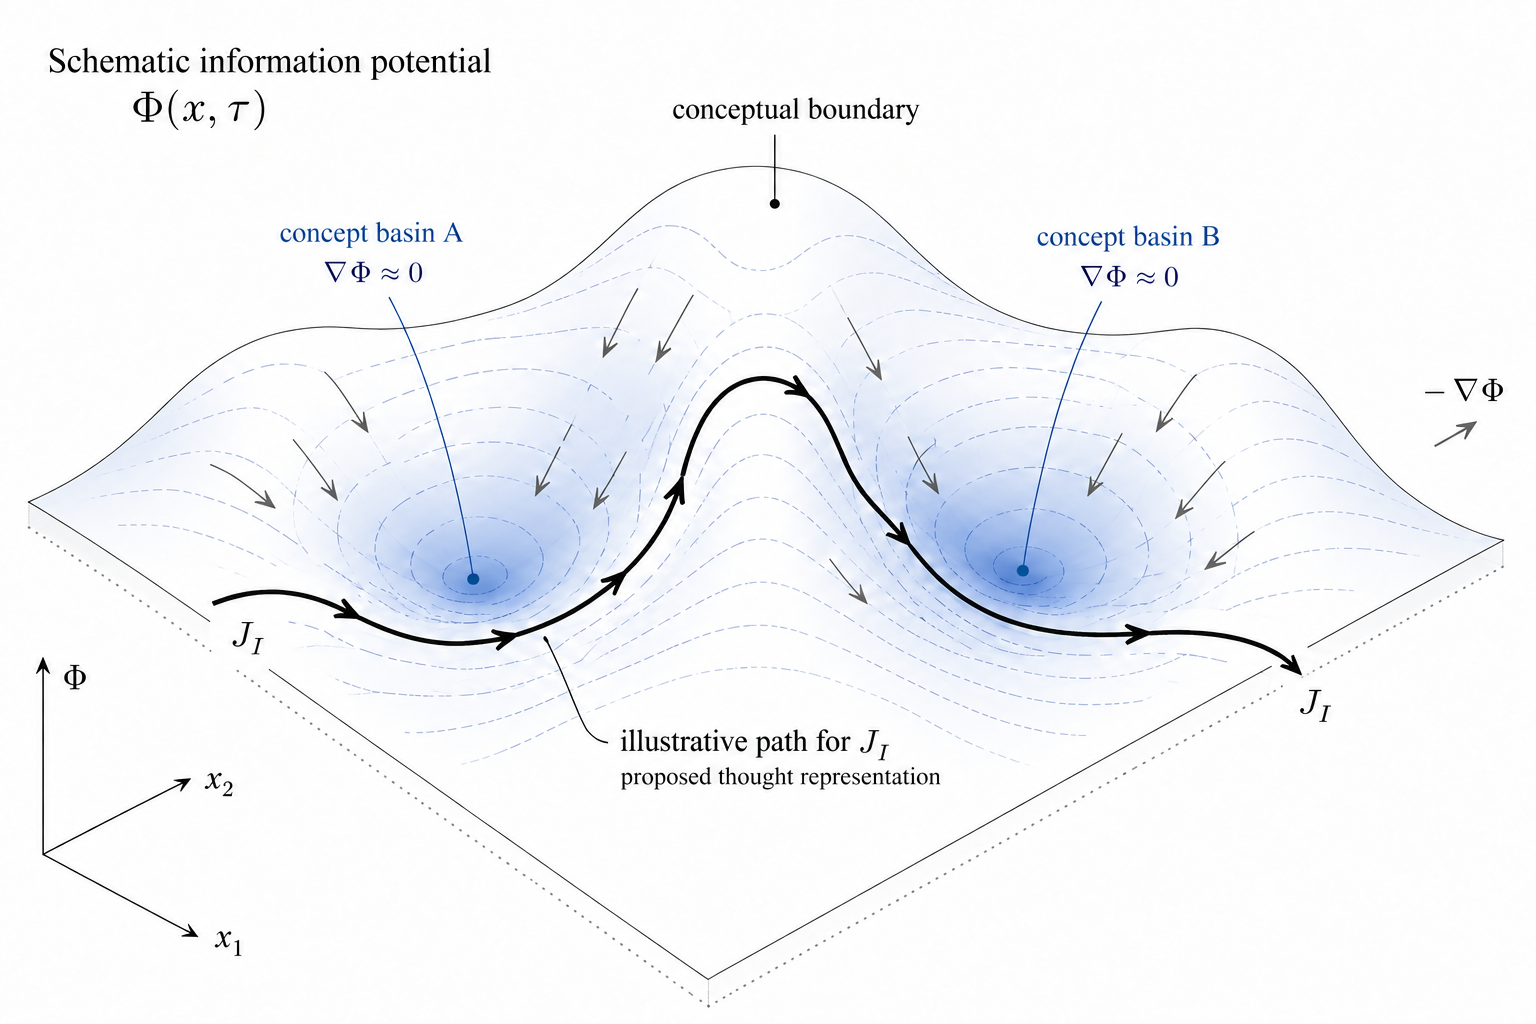
\includegraphics[width=0.92\linewidth]{figures/fig1_potential_geometry.png}
\caption{
情報ポテンシャルの幾何としての概念地形の模式図。
曲面はモデルのポテンシャル$\Phi(x,\tau)$を例示する。
盆地は$\nabla\Phi \approx 0$となる局所的な概念の定義を描く。
描かれた経路は流れ場$J_I$に関連づけた例示的な表現であり、場そのものでも、測定された思考経路でもない。
認知的な読みは提案であり、尾根はモデルレベルの概念境界を例示する。
}
\label{fig:potential-geometry}
\end{figure}

地形は、情報流$\JI$に関連する履歴形成的な幾何として、情報ポテンシャル$\Phi(x,\tau)$をモデル内で読むものである。
移動は$\JI$に関連する軌道表現であり、$-\nabla\Phi$は方向的な偏りを与えるが、経路全体を指定しない。
この移動を思考と呼ぶことは、さらに認知的解釈を加えることであって、場・経路・内容の同一性を意味しない。
理解の描像では、以前は困難だった領域での$|\nabla\Phi|$の局所的な減少を用いる。
感じられる容易さとの対応は仮説に留まる。形式的な閾値定義は、理解した感覚の独立した証拠ではない。

\subsection{谷としての概念}
この描像では、概念はポテンシャル地形の谷である。
それは$\Phi$が低く、軌道が自然に引き寄せられる領域である。
谷の深さには反復的な通過が反映されると提案し、幅はその概念が適用される文脈の広がりと比較する。
これらの比較は、独立した意味の測定を与えるものではない。

重要なのは、谷の中に意味が入っているわけではないという点である。
谷を\emph{動的アトラクタ}、すなわちモデル内で後続の軌道に偏りを与える領域として記述し、思考のパターンをその認知的解釈として提案する。
この枠組みで概念の「意味」と呼ぶものは、アトラクタが利用可能にする軌道の集合である。

\subsection{地形を形づくる操作としての言語トークン}
言語トークンは、自然言語の単語だけでなく、局所的な摂動として場に作用しうる、離散的で再アドレス可能なあらゆる媒体を含む広い意味で用いる。
記号、紋章、身振り、図、数式表記などが含まれる。
この記述では、それらに内在的な意味を割り当てない。
地形に偏りを与える局所的な摂動としてモデル化する。
類似した文脈での反復使用は、関連する谷を深めると仮定し、再利用の減少は浅化と関連づける。
送り手と受け手の地形がより似ていれば、摂動への反応もより似たものになりやすいと提案する。
地形の乖離は、コミュニケーションの失敗に寄与する可能性がある。
この比較仮説は、コミュニケーションの説明を尽くすものでも、コミュニケーションの成功から幾何を推定するものでもない。

\subsection{見えないGPU}
見えないGPUという比喩は、地形を直接調べることなしに認知を構造的に解釈する提案である。
思考が自然に浮かぶこと、つながりが自ずと示唆されること、理解が段階的に組み立てられるのではなく突然訪れること、といった経験例の整理に用いる。

これらの経験には、幾何の中に保存された内在的な意味ではなく、$\Phi$の幾何との対応を提案する。
これは主観的経験がどのように生成されるかの説明ではない。

以下の節では、この直観的語彙を形式的定義、および未解決の認知的・現象的対応写像から区別する。

\section{形式的対応}
\label{sec:formal}

本節ではVED$\times$IFGTの変数と概念的現象との対応の提案を記録する。
表は形式的役割とモデル内の解釈を分けるものであり、操作的な対応写像を与えない。
Master Variable Table v2.1への帰属には、本論文の冒頭で述べた出典の来歴に関する制限が残る。

\subsection{背景場}
情報密度場$I(x,\tau) = f(1-C(x,\tau))$を、概念構造のモデルにおける連続場として用いる。
本論文の$I$は、新しい認知的原始概念ではなく、IFGTの情報密度という語彙を認知的観測窓で解釈する提案であり、型を明示して確立された同一性ではない。
この局所的な解釈では、$I$は位置$x$、発展パラメータ$\tau$における未解決の情報的緊張の密度を表す。
それは、完全には安定化せず、完全には散逸していない準閉包領域として記述される。

高い$I$には概念的に活動的な領域との対応を、低い$I$には構造が大部分閉包した領域との対応を提案する。
これは較正された活動指標ではない。
本記述では、厳密な正値性$I(x,\tau)>0$を、通常の概念状態としての完全閉包を排するものと解釈する。
それだけで局所的な非ゼロの勾配や流れが保証されるわけではない。
勾配形成における残留非対称性、不均一な履歴、境界構造の役割は、モデルレベルの仮説に留まる。

情報ポテンシャル
\begin{equation}
  \Phi(x,\tau) = (K * I)(x,\tau)
  \label{eq:Phi_primary}
\end{equation}
が主要な幾何的対象である。
これを地形と読むことは、蓄積された偏りに対するモデルレベルの解釈である。
ポテンシャル勾配は有効な方向的偏りを与えるが、流れの関係には拡散項も含まれるため、それだけで完全な軌道を決めない。
場から軌道、軌道から思考への対応は、型を明示した写像や操作的な写像としては与えられていない。

\subsection{変数対応表}
\begin{center}
\renewcommand{\arraystretch}{1.5}
\begin{tabular}{p{0.22\textwidth}p{0.46\textwidth}p{0.22\textwidth}}
\toprule
\textbf{VED$\times$IFGT変数} &
\textbf{概念領域での解釈} &
\textbf{形式的役割} \\
\midrule
$C(x,\tau)$ & $x$における概念的固定の度合い & 背景場；$C \in [0,\Cmax)$ \\
$I(x,\tau) = f(1-C)$ & 未解決の概念的緊張の密度 & 中心となる場；常に$I > 0$ \\
$\Phi = K*I$ & モデル内の概念地形 & ポテンシャル幾何 \\
$\nabla\Phi$ & 認知的抵抗の低い側への偏りの提案 & $\JI$への拘束力 \\
$\JI = -D\nabla I + \mu F_I$ & 思考の表現の提案 & 形式的な流れ場 \\
$\sigma = \sigma_d - \sigma_p - \sigma_b$ & 地形の変形率 & 源項 \\
$\Delta$ & 新たな経験、知覚、言語入力 & 駆動源 \\
$\delta I$ & 未解決の概念的残差 & $I$を構成する痕跡 \\
$\tau$ & 経験的時間との対応の提案 & 形式的な発展・順序パラメータ \\
$\ell_i = \mathcal{Q}[I,\Phi,C;\cdot]$ & 再利用可能な言語トークン（自然言語の単語、記号、紋章、身振り、図、数式、または局所的な摂動として場に作用しうる任意の離散単位） & $\Phi$への作用の提案；シグネチャは未解決 \\
$\Phistar$ & 成熟した沈殿済みの概念地形 & $\Phi$の長時間アトラクタ \\
$\Cmax$ & 理想的な完全閉包境界 & 境界の表現であり、通常の状態ではない \\
\bottomrule
\end{tabular}
\end{center}

時間パラメータは形式的発展を順序づける。その経験的な読みは別の提案であり、時計の較正ではない。
同様に、沈殿した地形と長時間アトラクタという呼称には、第\ref{sec:core}節で論じる極限と履歴依存的解釈の未解決性が残る。

\begin{remark}[記法上の注意]
作用素$\mathcal{Q}$を量子化作用素と呼ぶのは、連続場の配置から離散的で再アドレス可能な単位を抽出するというその作用を、連続変数から離散値への移行と構造的に比較するためである。
これは非形式的な類比であって、数学的な同型や共通の物理的操作ではない。
CT内では「量子」という語を理論的主張として用いないが、この類比は作用素の名称に保持する。
\end{remark}

\subsection{この対応が主張しないこと}
以上の提案的対応は、意味内容、志向性、心理状態を形式体系へ導入するものではない。
特に、
\begin{itemize}
\item $\Phi$は意味場ではない。モデル内の相対的な遷移コストを記述するための動的な拘束幾何である。
\item $\JI$は思考内容ではない。それは形式的な流れ場であり、軌道の記述とその思考としての解釈は異なる使い方である。
経験に現れる内容は下流の主題として扱い、これらの使い方を同一視することで確立される帰結とはしない。
\item $\ell_i$は意味の単位ではない。$\nabla\Phi$へ局所的に結合する、離散的で再アドレス可能な単位である。
\end{itemize}
これらの除外は方法論上の必要事項であり、意味や経験の究極的な本性についての主張ではない。

\section{基本方程式}
\label{sec:core}

\paragraph{形式的範囲と未解決の仮定}
定義域、幾何と測度、パラメータの範囲は完全には指定されていない。
関連するIFGTの定式化にある追加の仮定や慣例は、正規化の選択も含め、CTへの特殊化条件として自動的には採用しない。
以下の範囲に関する記述は、欠けている仕様を示すものであり、それを補うものではない。

\subsection{場の発展}
ここでは収支関係を、モデルレベルの形式的テンプレートとして用いる。
定義域、初期条件・境界条件、正則性、正値性の保存条件を含む完全な初期境界値問題は指定していない。
この関係を用いることは、存在、一意性、適切性の確立を意味しない。
\begin{equation}
  \frac{\partial I}{\partial\tau} + \nabla\cdot\JI = \sigma,
  \label{eq:I_evolution}
\end{equation}
ここで情報流は
\begin{equation}
  \JI = -D\nabla I + \mu F_I, \qquad F_I = -\nabla\Phi = \alpha\nabla C,
  \label{eq:JI}
\end{equation}
である。力の関係において、最初の等号は負のポテンシャル勾配から有効力を定義する。
続く閉包勾配との等式は、局所的・有効な特殊化を意図したものであり、一般的な場の関係として保持する主要な畳み込みからの導出ではない。
この特殊化が有効となる近似領域と仮定は、今後確定する必要がある。

生成項は次のように分解する。
\begin{equation}
  \sigma = \sigma_{\mathrm{drive}} - \sigma_{\mathrm{dissip}} - \sigma_{\mathrm{barrier}}.
  \label{eq:sigma}
\end{equation}

三つの寄与は次のとおりである。
\begin{align}
  \sigma_{\mathrm{drive}}  &= a\Delta\!\left(1 - \frac{C}{C_*}\right),
  \label{eq:sigma_drive}\\
  \sigma_{\mathrm{dissip}} &= \Gamma C,
  \label{eq:sigma_dissip}\\
  \sigma_{\mathrm{barrier}}&= \frac{\kappa_B}{\Cmax - C}.
  \label{eq:sigma_barrier}
\end{align}

ここで$C_*$は観測窓内における概念的準閉包の有効飽和スケールを、$\Cmax$は理想的な完全閉包境界を表す。
概念的領域では一般に$C_* < \Cmax$である。

以下は有効な認知的解釈であり、測定された機構ではない。
$\sigma_{\mathrm{drive}}$は新たな入力（知覚、言語的摂動、報酬信号）の流入を表す。
$\sigma_{\mathrm{dissip}}$は未解決の緊張の自然な減衰（忘却、馴化）を表す。
$\sigma_{\mathrm{barrier}}$は概念的な過閉包に対する、投影的または粗視化された有効抵抗を表す。
これは基礎的な外部からの禁止として読むべきではなく、VEDとIFGTで用いられる有効障壁の記法に対する、認知領域での類似物である。
逆数の形だけでは、示された上側境界に動的に到達できないことは証明されない。
逆数表式の発散と全発展のもとでの不変性は別の主張であり、端点での振る舞いも不変領域の条件も、ここでは確立されていない。

\subsection{トークンと場の結合}
本構成では、離散的で再アドレス可能な構造を、安定で低コストな再帰のために提案する要件として扱う。
その動機は、連続場の配置を再訪することにはコストがかかり、ドリフトが生じやすい可能性にある。
連続系一般について不可能性を主張するものではない。
再アドレス可能性は、複雑な状態の再利用を支えることを意図している。
図\ref{fig:token-field-coupling}は結合仮説の例示であり、その帰結を実行によって示したものではない。

\begin{figure}[t]
\centering
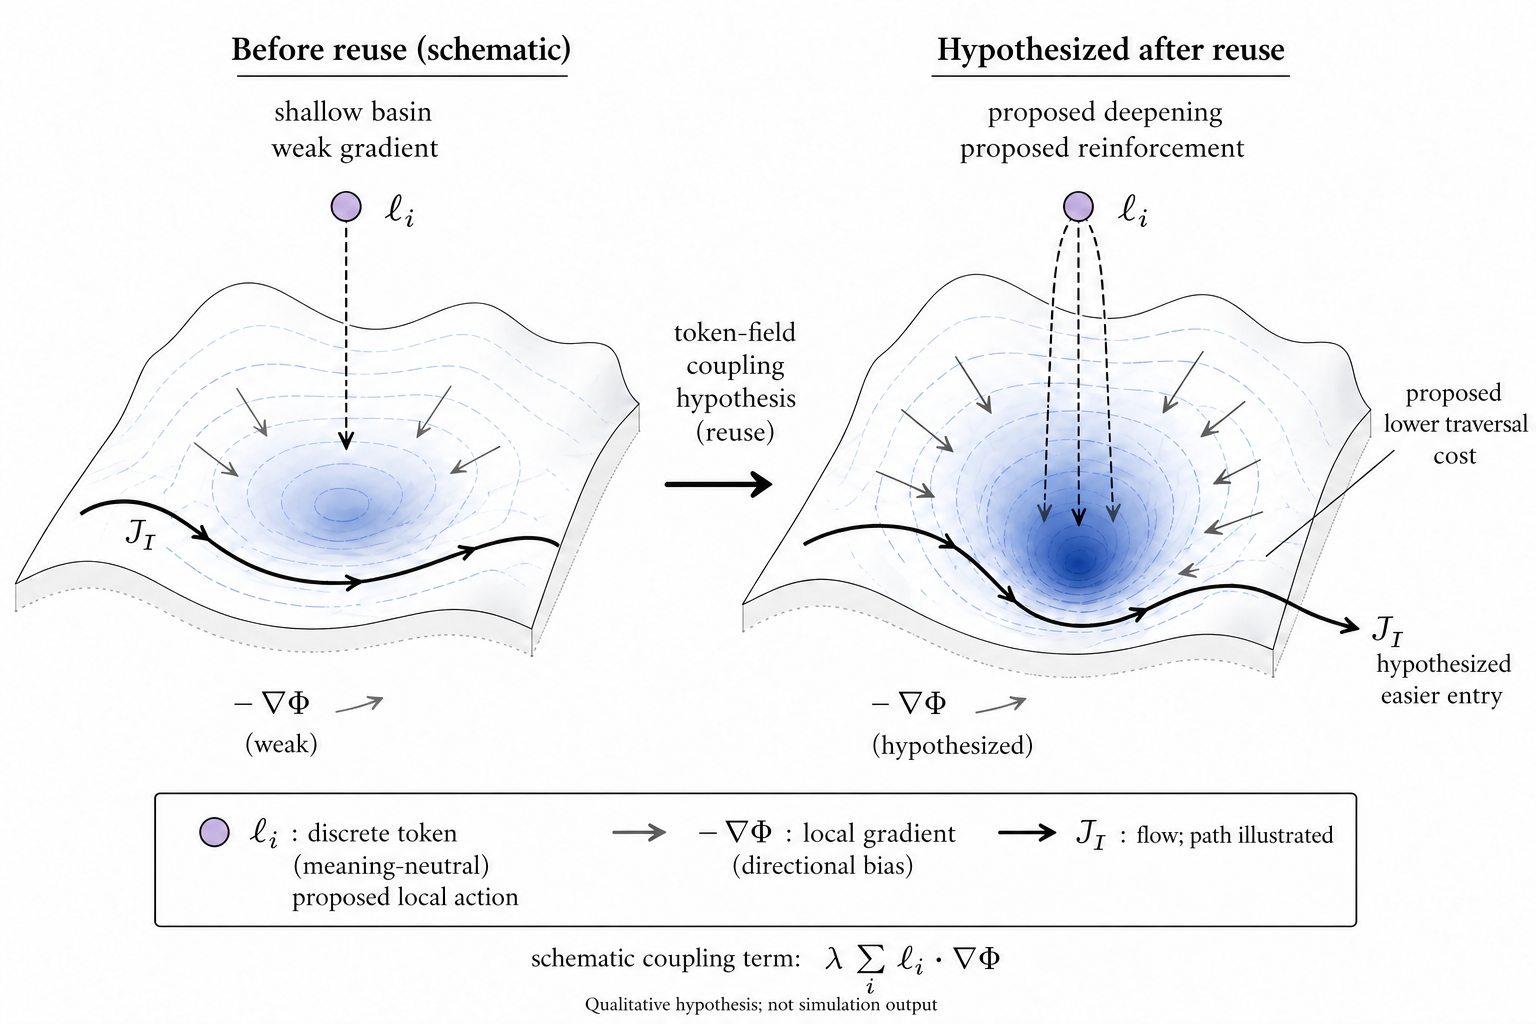
\includegraphics[width=0.95\linewidth]{figures/fig2_token_field_coupling.png}
\caption{
トークンと場の結合仮説の模式図であり、シミュレーション出力ではない。
離散トークン$\ell_i$には内在的な意味を割り当てず、$\nabla\Phi$への提案的な局所結合を動機として図示する。
$J_I$に関連する経路についての深化と通過コスト低下は仮説的効果であり、実行済みまたは導出済みの結果ではない。
表式$\lambda \sum_i \ell_i \cdot \nabla\Phi$は模式的なものに留まり、トークンの実現とペアリングは未解決である。
}
\label{fig:token-field-coupling}
\end{figure}

この構造を可能にする媒体は言語場である。
ここで「言語」は自然言語に限定せず、局所的な摂動として場に作用しうる、離散的で再アドレス可能なあらゆる媒体を広く含む。
記号、紋章、身振り、図、数式表記などが該当する。

言語トークン$\ell_i$（そのような任意の媒体から取られる離散単位）には、次の有効なトークン・場結合表式を割り当てる。
\begin{equation}
  \mathcal{L}_{\mathrm{eff}} = \mathcal{L}_{\mathrm{field}}[I]
  + \mathcal{L}_{\mathrm{token}}[\ell]
  + \lambda \sum_i \ell_i \cdot \nabla\Phi.
  \label{eq:coupling}
\end{equation}

提案する結合の役割は意味的なものではなく動的なものである。
トークンは意味を符号化せず、反復的な相互作用を通じて$\Phi$の局所的な発展に偏りを与えると仮定する。
勾配の強化と井戸の深化は定性的な機構仮説であり、項を書くだけで確立される帰結ではない。
結合表式は、離散トークンの数値的・ベクトル的実現と、ドット記法が示唆するペアリングに関して模式的なままであり、いずれも形式的には指定されていない。
有効・場・トークンの各ラグランジアン項の数学的な種類と、結合パラメータの仕様も未解決である。
ここでは、この表式からEuler--Lagrange方程式や、その他の変分・更新ダイナミクスを導出しない。

\subsection{沈殿と概念地形の形成}
以下の長時間表式は、反復的なトークンと場の相互作用の沈殿テンプレートとして保持し、確立された収束結果とはしない。
図\ref{fig:minimal-recursive-loop}は、枠組みの不可逆的順序という前提とともに、提案するフィードバック構成をまとめる。

\begin{figure}[t]
\centering
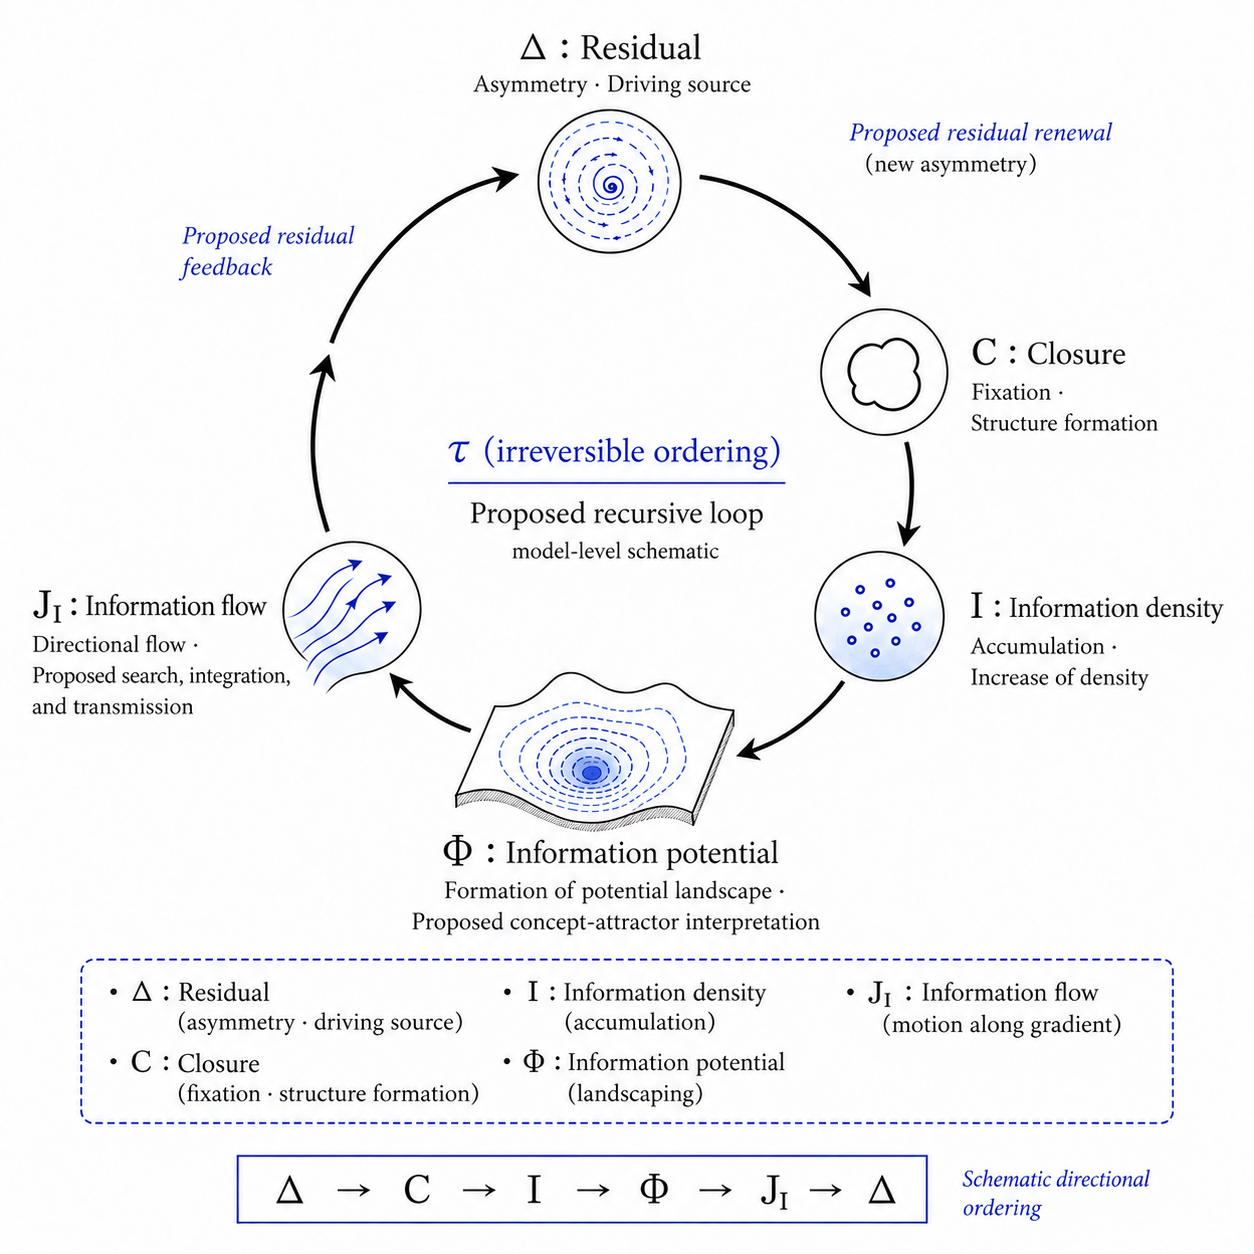
\includegraphics[width=0.82\linewidth]{figures/fig3_minimal_recursive_loop.png}
\caption{
VED$\times$IFGTの語彙による再帰ループの提案。
模式的な系列
$\Delta \to C \to I \to \Phi \to J_I \to \Delta$
は、残留非対称性$\Delta$、閉包$C$、情報密度$I$、ポテンシャル構造$\Phi$、情報流$J_I$を、提案するフィードバック構成の中で結びつける。
順序パラメータ$\tau$はモデルの不可逆的順序という前提を表す。
矢印は因果性の証明でも、実行された動的過程の実証でもない。
}
\label{fig:minimal-recursive-loop}
\end{figure}

\begin{equation}
  \Phi(x,\tau) \;\xrightarrow{\;\tau\to\infty\;}\; \Phistar(x).
  \label{eq:sedimentation}
\end{equation}

この矢印は長時間テンプレートであり、収束の様式は指定されていない。
以下の履歴解釈には、形式的な未解決性と出典・版に関する未解決性が残る。
表示された極限対象と、新たな入力による継続的な再形成との関係は、ここでは決定しない。
以下の非一意性・非静的性に関する表現は版に依存しており、その差を解消するために特定の解釈を選択しない。

$\Phistar$は沈殿した概念地形である。
それは必ずしも一意または静的ではなく、過去のすべての相互作用の履歴を反映し、新たな入力によって再形成され続ける。
ただし、地形が成熟するにつれてその速度は低下する。

\subsection{概念の定義}
\begin{definition}[概念]
位置$x$における\emph{概念}とは、次を満たす情報ポテンシャルの局所的安定領域である。
\begin{equation}
  \nabla\Phi(x) \approx 0, \qquad
  \text{with stability under small perturbations of } \JI.
  \label{eq:concept}
\end{equation}
$x$におけるポテンシャル井戸の深さには、変形への抵抗との構造的対応を提案する。
幅は文脈の広がりと比較する。これらの解釈は意味の較正ではない。
\end{definition}

\begin{definition}[理解]
概念領域$\mathcal{R}$を\emph{理解する}とは、$\mathcal{R}$を通る$\JI$の通過コストが、系に依存する閾値$\theta$より低くなっている状態である。
\begin{equation}
  \int_{\mathcal{R}} |\nabla\Phi|\,dx < \theta.
  \label{eq:understanding}
\end{equation}
ここで$\theta$は、再帰コストの許容範囲を表す、系に依存する有効閾値である。
具体的な値は$D$、$\mu$、$\alpha$および関連するパラメータを含む系の構造に依存し、本論文では指定しない。
理解は二値的な状態ではなく、$\Phi$の発展に伴って出入りしうる動的条件である。
\end{definition}

この定義は局所的なモデル状態を指定するものであり、独立した認知的・現象的基準ではない。
したがって、感じられる容易さとの提案的関係は別途評価しなければならない。
低コストな状態を定義することは、理解の経験を説明することではない。

\subsection{厳密な正値性制約}
厳密な正値性の記述は、モデルレベルの許容条件として保持する。
この正値域の制約、以下の正出力の前提、そして全収支発展のもとでの保存は、別々の形式的責務であり、ここではその正当化を確立していない。
この記述
\begin{equation}
  \boxed{I(x,\tau) > 0 \qquad \forall\,x,\,\tau,}
  \label{eq:positivity}
\end{equation}
は、$C < \Cmax$および$C < \Cmax$に対する正出力の前提$I = f(1-C) > 0$とともに述べられる。
ここで$\Cmax$は理想的な完全閉包境界を表し、概念系の通常の到達可能な状態ではない。

\begin{proposition}[通常の完全な概念的閉包の不在]
VED$\times$IFGTのモデル解釈内では、$I>0$は完全な概念的閉包を通常の動的状態から排する。
これとは別に、残留非対称性、空間的不均一性、境界構造を持つ非自明な地形では、$\Phi$のさらなる勾配と$\JI$の利用可能な方向が再び現れると提案する。
これは条件付きの分化仮説であり、正値性だけの帰結ではない。
閉包についての解釈は、正の$I$がすべて$\nabla\Phi\neq0$を持たねばならないという各点での数学的主張ではない。
追加条件なしでは、正値性だけから非ゼロの流れも含意されない。
完全な流れにはポテンシャル勾配の寄与以外も含まれる。
\end{proposition}

\begin{remark}
このモデルレベルの区別は、知性と理解との比較を動機づけるものであり、それらを正値性から導出するものではない。
安定アトラクタは局所的に静穏に見えることがある。
新たな摂動や、より広い観測窓のもとでは、さらなる分化が可能であり続けると提案する。
無条件の学習や革新の保証は推論しない。
\end{remark}

\section{構造的解釈}
\label{sec:structural}

\subsection{構造クラスの候補}
VED$\times$IFGT枠組みは、以下の構造クラスの候補と認知的解釈を動機づける。
表はモデルに基づく分類を整理するものであり、形式的な存在定理や分類定理ではない。
詳細な解の解析と独立した認知的対応は今後の課題である。

\begin{center}
\renewcommand{\arraystretch}{1.5}
\begin{tabular}{p{0.29\textwidth}p{0.31\textwidth}p{0.30\textwidth}}
\toprule
\textbf{候補クラス} & \textbf{場の構造} & \textbf{認知的解釈} \\
\midrule
滑らかな勾配領域 & $\nabla\Phi$が緩やかに変化 & 背景的な認知的傾向 \\
浅い準安定井戸 & $\nabla\Phi\approx 0$、深さが小さい & 暫定的または不安定な概念 \\
深い安定井戸 & $\nabla\Phi\approx 0$、深さが大きい & 定着した概念や信念 \\
リミットサイクル軌道 & $\JI$が沈殿せず循環 & 反復する思考パターン \\
障壁領域 & $|\nabla\Phi|$が大きい & 認知的な行き詰まりや抵抗 \\
尾根構造 & $\Phi$の局所最大 & 概念境界やカテゴリの縁 \\
\bottomrule
\end{tabular}
\end{center}

\subsection{深さ、幅、頑健性}
三つの幾何的パラメータが概念アトラクタを特徴づける。

\textbf{深さ}（井戸内の$-\min\Phi$）には、新たな入力による変形への抵抗との対応を提案する。
深い井戸を抵抗の強い概念と、浅い井戸を変位しやすい概念と比較する。

\textbf{幅}（閾値未満の領域の空間的広がり）は、文脈の範囲と比較する。
広い井戸を適用範囲の広さと、狭い井戸を文脈依存性の高い概念と比較する。

\textbf{頑健性}（極小点における$\Phi$の曲率）は、精密さの比較指標として提案する。
高い曲率を鋭い概念と、低い曲率を曖昧または多義的な概念と定性的に関連づける。
これらの意味的属性は、いずれも幾何的記述だけでは較正されない。

これらの幾何的属性は、固定された内在的性質として扱わない。
式\eqref{eq:I_evolution}--\eqref{eq:sigma_barrier}の関係のもとで、$\Phi$とともに発展するものとしてモデル化する。

\subsection{概念境界}
$\Phi$の尾根構造、すなわち隣接する井戸を隔てる局所的に高いポテンシャルの領域は、この記述では概念間の区別である概念境界を表す。
境界は鋭い線ではなく、通過コストの高い広がりを持った領域である。

定性的な仮説は、反復的な言語的・経験的摂動のもとで概念境界が移動しうる、というものである。
尾根近傍で結合するトークンは、尾根を強化して区別を深めたり、侵食して隣接概念を融合させたりすると提案する。
これは意味ドリフトと概念変化の動的記述の候補であり、確立された認知機構や意味の対応写像ではない。

\subsection{語彙の選択と分布的記述}
安定化したトークン$\{\ell_i\}$の全体集合を、この枠組みでは語彙と呼ぶ。
以下の表式は安定性によって集合を選ぶものである。
語彙が場に分布するという広い記述によって、その集合が確率分布になるわけではない。
\begin{equation}
  \mathcal{V} = \bigl\{\ell_i \;\big|\; S(\ell_i) > \epsilon \bigr\},
  \label{eq:vocabulary}
\end{equation}
ここで$S(\ell_i)$は、再利用頻度、持続時間、盆地の深さに依存することを意図した安定性汎関数であり、$\epsilon$は系に依存する閾値である。
ここでは、この汎関数と閾値に抽出規則や較正規則を与えない。

語彙は、使用によって再形成される、場に関連した組織化として解釈する。
トークン頻度には盆地のアクセス可能性との関係を提案するが、意味的重要性の尺度とはしない。
曖昧で文脈依存的な区別は、この解釈的描像の一部であり、トークンの操作的基準ではない。

\section{ダイナミクス}
\label{sec:dynamics}

\subsection{沈殿}
沈殿とは、反復的なトークンと場の相互作用のもとで井戸が深まり、概念が安定化するという提案的過程の呼称である。
以下の三段階は機能的なフィードバック構成を記述するものであり、実行された動的過程の実証ではない。
最初のトークン・盆地の立ち上がりと、結合の更新上の帰結は未解決である。

\textbf{段階1：初期摂動。}
提案するシナリオでは、新たな入力$\Delta$を、$\sigma_{\mathrm{drive}}$のスパイク、$I$の局所的増加、一過性のポテンシャル勾配と関連づける。
情報流$\JI$は摂動に応答するものとしてモデル化するが、これは再構成された思考経路ではない。

\textbf{段階2：強化。}
類似入力へのその後の接触や、内的な再帰的活性化によって摂動が繰り返されると、$\Phi$の局所勾配が強化されると仮定する。
井戸の深化はトークンと場の結合\eqref{eq:coupling}の提案的効果であり、個々の再利用や表式だけによって保証される結果ではない。

\textbf{段階3：安定化。}
提案する安定化段階では、井戸の深化を通過コストの低下と、その後の再利用をさらなる強化と関連づける。
自己維持する概念は、このように得られる維持仮説であり、フィードバック構成から実証された帰結ではない。

\subsection{忘却}
ここでは忘却を、再利用頻度が低下すると$\Phi$がより平坦な配置へ緩和することとの類比で解釈する。
既存の散逸項を形式的テンプレートとして保持する。
\begin{equation}
  \sigma_{\mathrm{dissip}} = \Gamma C.
\end{equation}
このモデル描像では、アクセス可能性の低下を、保存された記号の消去ではなく、安定性の再分配と関連づける。
浅くなる井戸では通過コストが高まると提案する。
これは、忘れられた概念が決して消滅しないことを確立しない。
再活性化（想起）も、再開されたトークンと場の相互作用を通じた再深化としてモデル化するが、普遍的な記憶機構とは同一視しない。

\subsection{概念変化}
確立された概念の意味、範囲、適用の変化である概念変化を、ここでは$\Phistar$の変化を用いて表現する。
二つの井戸の融合、一つの井戸の二つへの分裂、地形内での変位などである。
これらの幾何的選択肢は認知的対応の提案を整理するものであり、長時間対象を確定したり、トポロジーから認知への写像を証明したりするものではない。

この候補となる記述では、そのような変化を既存アトラクタの深さに対する持続的摂動と関連づけるが、信念改訂の較正された必要条件や十分条件とはしない。
有効障壁項$\sigma_{\mathrm{barrier}}$は、この有効記述において保護的な役割を担う。
$C\to\Cmax$となるにつれて、抵抗という解釈を、深く定着した概念を変える困難さの増大と比較する。
これは概念的観測窓内の過閉包に対する有効記述として理解すべきであり、外部から課された壁ではない。
この記述は信念改訂への抵抗についての候補となる説明を与えるが、逆数項は認知的な禁止を確立しない。

\subsection{洞察と急速遷移仮説}
問題が解けた、あるいは離れていた考えが結びついたという突然の感覚は、$\Phi$の局所トポロジーの急速な変化との対応の提案を動機づける。
井戸の融合や障壁の崩れは、分岐に似た表現を与える。
幾何的遷移、認知的な問題解決、感じられる出来事は別々の主張であり、ここでは分岐定理も独立した認知的終点も与えない。

突然性の主観的感覚には、摂動の蓄積に続いて急速な遷移が起こるという閾値描像との対応を仮定する。
この描像は、知覚的閾値を独立に同定するものでも、遷移と名づけるだけで感じられる突然性を説明するものでもない。

\section{スケール反転：個体から社会へ}
\label{sec:multiscale}

\subsection{機能と支配的コストの比較}
前節までのモデルは、個体の認知系のレベルで解釈している。
その解釈では、状態を再訪することと、再利用可能な離散的な手がかりで連続配置を表現すること、すなわち再帰と圧縮を支配的なコストとして提案する。
こうした構成上の仮定のもとで、言語トークンに内部制御の役割を割り当てる。

この役割を相互作用するエージェント間の同期・協調と比較することで、社会的拡張を提案する。
トークンは共有軌道の安定化を助け、他のエージェントの反応についての不確実性を減らすと仮定する。
表は提案する支配的コストとトークンの機能を対比するものであり、個体と集合のダイナミクスが同一であることを確立しない。

\begin{center}
\begin{tabular}{lll}
\toprule
\textbf{スケール} & \textbf{支配的コスト} & \textbf{トークンの機能} \\
\midrule
個体 & 再帰、圧縮 & 内部制御単位 \\
社会 & 同期、協調 & 共有地形のアンカー \\
\bottomrule
\end{tabular}
\end{center}

この比較は、異なる有効制約のもとで類似した再アドレス機能を提案する。
スケールをまたいでトークンの性質が不変であることを確立するものではない。
集合的な集約、共通の状態空間、型を明示した翻訳は未指定であり、同じ記法の再利用から共有場の測定が得られるわけではない。

\subsection{社会的な概念地形}
社会的仮説では、事前の地形が十分に類似しているとき、共有された言語入力への反復的な接触を、相関した井戸の深化と比較する。
共有概念地形は、この提案された組織化に対するモデルレベルの名称である。

この描像では、共有地形は一人のエージェント内に保存されるのではなく、エージェント間に分布し、継続的な言語的相互作用を通じて維持される。
履歴によって形成された集合的幾何は、これらの相互作用の解釈であり、測定された集合場ではない。

\subsection{規範、制度、パラダイム}
深く沈殿した社会的領域を、規範、制度、科学的パラダイムと構造的に比較する。
このアトラクタ類比では、集合的な$\Phi$を用いて持続を表現するが、制度と形式的アトラクタの同一性を主張しない。

別の仮説として、深さを安定性と逸脱コストに、協調した摂動を制度変化に関連づける。
これは中央による強制を唯一の説明とせずに持続を考える方法を提供するものであり、強制が不要であることの証拠ではない。
パラダイム転換の歴史的困難さは比較対象の候補であって、井戸の深さによって説明された結果ではない。
独立した制度の基準と深さの推定は未解決である。
安定性を深さの定義と、その説明上の役割を支える独立した証拠の両方に用いることはできない。

\subsection{地形維持としての知性}
この社会的スケールの記述内では、提案する分散的過程に対して局所的な機能上の呼称を用いる。
\begin{quote}
\itshape
ここでいう社会的知性とは、言語を通じた概念地形の分散的な維持、同期、再形成の呼称である。
\end{quote}

この命名は、知性の確立された一般的定義や生成ではなく、個体の知性を排するものでもない。
repository内のIntelligence諸理論との関係は、概念的な引き継ぎであって、下流の研究から検証を移し入れるものではない。

個々のエージェントは、この過程の一時的な参加者としてモデル化する。
地形を通過し、局所的な変形を導入し、外在化された言語ログを通じて安定化した構造を後続のエージェントへ伝える。

厳密な正値性$I>0$は、提案された社会的地形について類比的な非閉包の読みを動機づけるものであり、集合的ダイナミクスの導出ではない。
さらなる分化と革新は、残留非対称性を再活性化する新たな摂動や、より広い観測窓のもとで提案する可能性であり、正値性だけで保証される結果ではない。

\section{病理的描像と限界}
\label{sec:pathologies}

\subsection{意図的に除外するもの}
本枠組みは以下を意図的に除外する。

\textbf{意味理論。}
指示、真理条件、解釈内容については主張しない。
意味という語が現れる場合、それは安定した軌道に適用される創発的な呼称であり、理論の原始概念ではない。

\textbf{現象学と意識。}
本枠組みは主観的経験を生成せず、説明もしない。
意識的アクセスは、現在repository内にsourceが存在するConsciousness Theoryとの比較に向けた、下流の主題として扱う。
この比較は、CTに機構を移し入れるものでも、その現象的解釈を検証するものでもない。

\textbf{神経生物学的実装。}
本理論は、特定の神経アーキテクチャに依存しない抽象度で、構造的・動的条件を記述する。
神経実装との対応は今後の課題とする。

\subsection{失敗領域の提案}
以下は定性的な領域仮説であり、診断的・臨床的分類器でも、認知状態の必要条件や十分条件でもない。

\textbf{過閉包（深すぎる井戸）。}
$\sigma_{\mathrm{drive}}$に比べて有効な$\sigma_{\mathrm{barrier}}$が大きいことを、地形変化に抵抗する領域として解釈する。
提案する認知的対応は、より反復的で適応性の低い思考である。
硬直性、教条性、定着した信念は、ここでは現象学的な比較の語であり、パラメータによって同定または因果的に説明された状態ではない。

\textbf{閉包不足（浅すぎる井戸）。}
$\sigma_{\mathrm{dissip}}$の優勢を、モデル描像では井戸の形成より速い浅化と関連づける。
これに不安定な思考や概念の安定化の困難さとの対応を提案する。
理解の持続性の低さとの関係は定性的な仮説であり、持続を阻む機構として確立されたものではない。

\textbf{同期の破綻（社会的スケール）。}
事前の地形の乖離、共有された接触の不足、意図的な操作は、エージェント間の同期を弱めると提案する。
共有地形の断片化は、このパターンのモデル解釈であり、コミュニケーションの失敗、文化的対立、認識的分極化との比較候補を与える。
これらの結果を一つの測定された領域と同一視したり、集合的幾何だけから推論したりするものではない。

\subsection{対象範囲の限界}
本理論は構造的・動的記述を提案するが、以下を確立しない。
\begin{itemize}
\item 特定の認知系についての定量的予測（そのためには$K$、$D$、$\mu$、$\alpha$、$\Gamma$、$\kappa_B$の具体的指定が必要である）。
\item $\Phi$の幾何と、観測可能な神経・行動データとの対応条件。
\item 言語獲得、意味変化、集合的知性の完全な理論。
\end{itemize}
これらは提案された枠組み内の今後の課題として残る。

\section{ノートシリーズとの関係}
\label{sec:note}

本論文のsourceは、沈殿、流れ、地形の語彙を用いる関連ノートシリーズ（L1層）に言及している。
正確なノート成果物、題名、版は未解決である。
表は、記録された語彙とモデル構造についてのCT自身の教育的比較を保持する。
独立に同定されたノートの検証済みの再構成でも、型を明示した写像でも、検証のための証拠でもない。
認知的・現象的な項目は解釈の提案であり、表示した対応によって確立された同一性ではない。

\begin{center}
\renewcommand{\arraystretch}{1.5}
\begin{tabular}{p{0.40\textwidth}p{0.52\textwidth}}
\toprule
\textbf{ここに記録されたノート語彙（J：日本語）} &
\textbf{提案するモデル対応} \\
\midrule
「ログの沈殿」 & $\sigma_{\mathrm{drive}}$を介した$\Phi$の深化 \\
「安定点」 & 局所的安定領域：$\nabla\Phi\approx 0$ \\
「概念のくぼみ」 & $\Phi$のポテンシャル井戸 \\
「全体勾配」 & 情報ポテンシャル$\Phi = K*I$ \\
「通りやすさ」 & $-\Phi(x,\tau)$（通りやすさが高い$=$$\Phi$が低い） \\
「谷」 & $\Phi$の深い井戸 \\
「壁」 & $\Phi$が高い尾根領域 \\
「理解した感覚」 & 通過コスト$\int|\nabla\Phi|dx$の低下 \\
「思考の癖」 & $\JI$のリミットサイクル軌道 \\
「GPU的な装置」 & $\JI$に対する$\Phi$の閾値未満の作用 \\
「言語粒子」 & $\nabla\Phi$へ結合する離散トークン$\ell_i$ \\
「圧縮」 & 量子化作用素$\mathcal{Q}$ \\
「社会的共有地形」 & エージェント間での社会的$\Phistar$の維持の提案 \\
\bottomrule
\end{tabular}
\end{center}

\subsection{この比較の限界}
ここに記録された記述は、未同定のノート成果物に検証済みの立場を帰属させることなく、非専門的な直観として用いる。
CTの立場では、それらは場理論的量の\emph{解釈}であり、定義ではない。

特に、
\begin{itemize}
\item 記録された意味の語彙は、反復的な通過とポテンシャル井戸の深さと比較する。
内在的な意味対象や、較正された意味尺度と比較するものではない。
\item 記録された「理解した感覚」の記述には、\eqref{eq:understanding}に関連する容易さの変化との対応を提案する。
局所的定義は、この現象的対応の独立した証拠ではない。
\item ここでConsciousnessのノートに帰属させているCPU/GPUの区別を、高速レーン／低速レーンの分解と比較する。
Consciousness Theoryには現在repository内のsourceがあるが、ノートと論文の正確な版の関係は未解決である。
これは構造的比較であり、共通量、型を明示した翻訳、実証された機構の移転ではない。
\end{itemize}

\subsection{L3 → L1の方向}
本論文（L3）はノートシリーズ（L1）を改訂したり置き換えたりしない。
ここでの寄与は解釈の整理であり、記録された直観を比較するためのモデル語彙であって、それらの理論的検証ではない。
正確な出典の帰属は未解決である。

地形、流れ、沈殿を場理論的対象と比較する。
理解、意味、思考はその語彙の別々の解釈的な読みであり、形式的な指示対象を割り当てることによって独立に説明されるものではない。
二つの説明層は、一方が他方の検証証拠となることなしに、相補的でありうる。

\section{考察}
\label{sec:discussion}

\subsection{既存の枠組みとの関係}
\textbf{認知への力学系的アプローチ。}
概念を力学系のアトラクタとして扱うことには、コネクショニズムや身体性認知の研究に先例がある\citep[e.g.,][]{thelen1994dynamic}。
本枠組みは、VEDとIFGTの有効な動的慣例から構造的な動機を得て、明示的なトークン・場結合表式を提案する。
このsourceの再利用は、認知的アトラクタを上流の公理から導出したり、その機構を確立したりするものではない。

\textbf{分布意味論。}
分布意味論との比較は概念的なものである。
共起に関連するトークン空間の幾何を、CTが提案する履歴依存的なトークン・場幾何と対比する。
CTは\emph{使用}を重視するが、使用と\emph{共起}が経験的に排他的であるとも、この比較によって優れた意味表現が確立されるとも主張しない。
ここではコーパス、埋め込みの距離尺度、モデル間写像を与えない。

\textbf{予測処理と自由エネルギー。}
予測処理の記述は、認知を予測誤差の最小化として扱う\citep{friston2010free}。
ここでは概念的な比較を提案する。
$\sigma_{\mathrm{drive}}$は予測誤差の流入と並べて解釈でき、$\Phi$の井戸の深化は長期的な誤差最小化との類比で理解できる。
CTはこれらの量を予測誤差や自由エネルギーの変数と同一視しない。
ベイズ的生成モデルを採用するとは定めないが、その非採用は、より高い一般性や理論的包含の証明ではない。

\subsection{未解決問題}
\textbf{定量的対応。}
本枠組みは構造的記述を提案するが、畳み込み核$K$の具体的な形や、パラメータ$D$、$\mu$、$\alpha$、$\Gamma$、$\kappa_B$の値を指定しない。
これらを行動、言語、神経の経験的データから同定することは、主要な未解決問題である。

\textbf{トポロジーと概念の個体化。}
本枠組みは概念を$\Phi$の局所的安定領域として定義する。
しかし、ある領域が関連する概念の集まりではなく単一の概念と数えられる条件は、まだ指定されていない。
概念の個体化にはトポロジー的基準が必要である。

\textbf{マルチエージェントの同期ダイナミクス。}
社会的地形は定性的に記述している。
共有地形が安定に形成される条件や破綻する条件を含め、マルチエージェントのトークン・場相互作用を形式的に扱う方法は今後の課題である。

\textbf{神経実装との接続。}
場の量$I$、$\Phi$、$\JI$と、測定可能な神経量（発火率、結合重み、振動ダイナミクス）との対応は、経験的神経科学との協働を必要とする主要な未解決問題である。

\section{結論}
\label{sec:conclusion}

本論文は、VED$\times$IFGT枠組みの最初の応用層として、概念地形の場理論的記述であるConceptual Topography（CT）を展開した。

中心となる提案は、再帰的なトークンと場の相互作用のもとで履歴によって形成された情報場$I(x,\tau)$の幾何を、モデル内の概念地形として用いることである。
この呼称は、収束、認知機構、経験へのアクセスについての主張とは別である。
モデル内では、意味の原始概念、志向的状態、意味を担う単位は必要としない。

保持する定義と提案する解釈は以下のとおりである。
\begin{enumerate}
\item 概念は、摂動に対する安定性を伴う$\nabla\Phi\approx 0$によって定義される、情報ポテンシャル$\Phi = K*I$の局所的安定領域である。
その深さ、幅、頑健性は、相互作用の履歴とともに連続的に発展する動的量である。
\item 理解は概念領域の通過コストの低下であり、認識論的な達成ではない。
地形の発展に伴って、そこに入り、そこから出ることができる。
\item 言語トークンは、意味内容を担わずに$\nabla\Phi$へ結合する、離散的で再アドレス可能な単位として機能する。
低コストな再帰がこの構成上の役割を動機づける。
反復的な相互作用による深化は定性的仮説に留まり、結合の保証された帰結ではない。
\item モデル内では、厳密な正値性$I(x,\tau)>0$を、通常の完全な概念的閉包を排するものと解釈する。
局所的な静穏は許容する。
新たな摂動やより広い観測窓のもとでのさらなる分化は、条件付きの提案であり、正値性の各点での帰結ではない。
\item 社会的スケールでは、異なるコストのもとで比較可能なトークン機能が、共有地形仮説を動機づける。
規範、制度、パラダイムをアトラクタと比較する。
深さと安定性の関係は、独立した社会的基準を必要とする仮説に留まる。
集合的な維持は局所的な機能語彙であり、確立された知性の一般的定義ではない。
\end{enumerate}

本枠組みは関連ノートシリーズを改訂したり置き換えたりしない。
記録された直観とのCT内の教育的比較を保持するが、独立に同定されたノートを検証する支持とはしない。
ノートとMaster表の正確な出典・版の帰属は未解決である。

定量的なパラメータ同定、概念個体化のトポロジー的基準、マルチエージェントの同期ダイナミクス、神経的対応といった詳細な展開は、今後の課題である。
長時間対象、結合のシグネチャ、正値性の保存、その他の形式的OPEN問題は、文章の範囲を限定したことによって解決されたわけではない。
同様に、理解を感じられる容易さから、洞察を主観的突然性から分けたことは、いずれの対応も確立しない。

要するに、Conceptual Topographyは、VED$\times$IFGT枠組みに基づき、概念構造と認知機能の場理論的表現を提案する。
概念と物理的粒子は、同一の実体や還元可能な対象としてではなく、投影された安定化領域として比較しうる。
反復する生成文法は、この比較における発見的なモチーフであり、共通方程式の定理ではない。
深さ、幅、持続、観測窓は比較を整理するが、共通量、共通場、型を明示した翻訳を確立しない。
経験的検証や主観的経験の説明は主張しない。


% ---- bibliography ----
\bibliographystyle{plainnat}
\bibliography{refs}

\end{document}
